\documentclass{beamer}

\title{Exploring Semantic Hierarchies to Improve Resolution Theorem Proving on Ontologies}
\subtitle{Stanley Small}

\begin{document}
	\frame {
		\titlepage
	}
	
	\frame {
    	\frametitle{Outline}
    	\begin{itemize}
		    \item Background
	        \item Motivation
	        \item Related Work
            \item Methods
            \item Timeline
            \item Deliverables
            \item Completed Work
            \item Questions
        \end{itemize}
	}
	
	\frame {
	    \frametitle{Formal Logic}
	    Formal logic, specifically first-order logic, represents an environment using statements which can be used to form logical and mathematical proofs
	    
	    \[\forall x [isCat(x) \rightarrow hasFourLegs(x)]\]
	}
	
	\frame {
	    \frametitle{Theorem Proving}
	    Axioms are statements accepted without proof
        \[isMan(socrates)\]
        \[\lnot isMan(X)\lor isMortal(X)\]
	    A conjecture is an unproved statement believed to be true 
	    \[isMortal(socrates)\]
	}

	\frame {
		\frametitle{Resolution}
		Axioms must be expressed in Conjunctive Normal Form
		\[a \rightarrow c\]
		\[\lnot a \lor c\]
		One can then resolve the statements
		\[\frac{a \lor b, \lnot a \lor c }{b \lor c}\]
	}
	
	\frame {
		\frametitle{Resolution Tree}
		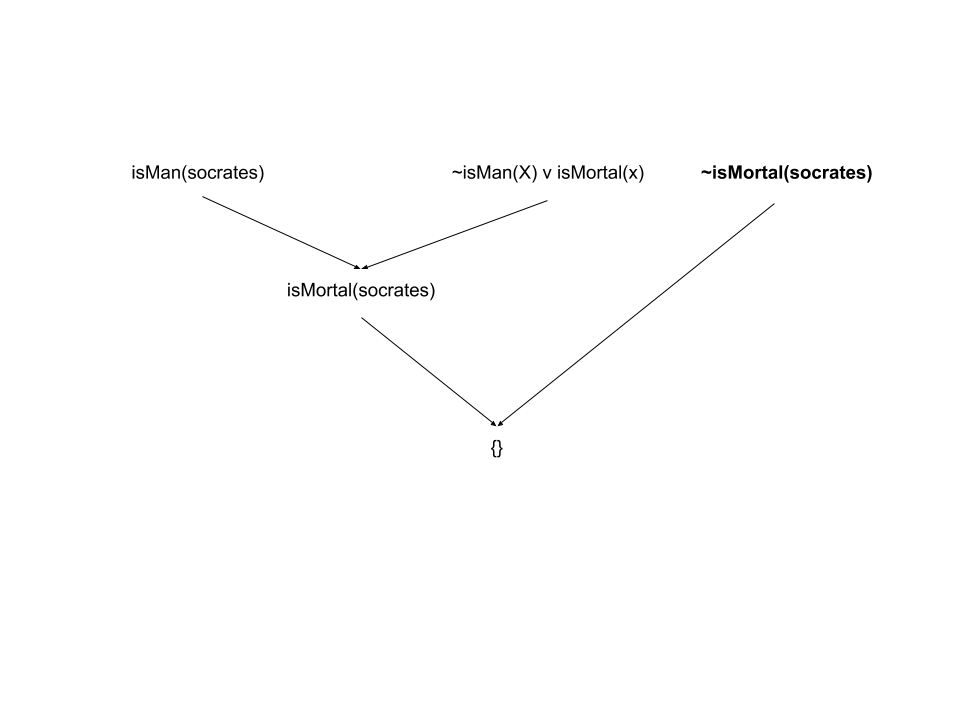
\includegraphics[scale=.3]{res_tree.png}
	}
	
	\frame {
		\frametitle{Resolution Theorem Proving}
        \begin{itemize}
            \item Search space increases exponentially with the addition of each new axiom
            \item Currently only the syntax of statements is taken into account
        \end{itemize}
	}
	
	\frame {
		\frametitle{Comparing Syntax to Semantics}
		\begin{itemize}
		    \item Syntax defines the structure of a sentence
		    \item Semantics describe the meaning of a sentence
		\end{itemize}

	}
	
	\frame {
		\frametitle{Knuth-Bendix Ordering}
		\begin{itemize}
		    \item Each predicate is assigned a weight
		    \item Terms are automatically assigned weights by summing the predicate weights
		\end{itemize}

	}
	
	\frame {
		\frametitle{Ontologies}
		An ontology defines categories and relationships among objects. Typically, the objects can be arranged in a hierarchy. 
		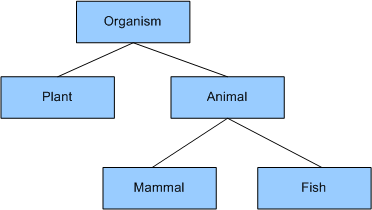
\includegraphics[scale = .5]{simple-hierarchy.png}
		
	}
	
	
	\frame {
		\frametitle{Objective}
		\begin{itemize}
		    \item Use semantic knowledge in addition to syntax of logical statements
		    \item Improve automated theorem proving
		    \item Possibly advance artificial intelligence research
		\end{itemize}

	}
	
	\frame {
		\frametitle{Related Work}
		\begin{itemize}
		    \item Prover-independent Axiom Selection for Automated Theorem Proving in Ontohub (Eugen, Till)
		    \item Premise Selection for Mathematics by Corpus Analysis and Kernel Methods (Alama, Jesse and Heskes, Tom and K{\"u}hlwein, Daniel and Tsivtsivadze, Evgeni and Urban, Josef)
		    \item Sledgehammer: Judgement Day (B{\"o}hme, Sascha and Nipkow, Tobias)
		\end{itemize}
	}
	
	\frame{
	    \frametitle{Prover-independent Axiom Selection for Automated Theorem Proving in Ontohub}
	    \begin{itemize}
	        \item An empirical study comparing two term-ordering methods
	        \item Quantitative analysis for percentage of proofs completed in a given time
	    \end{itemize}
	}
	
	\frame{
	    \frametitle{Premise Selection for Mathematics by Corpus Analysis and Kernel Methods}
	    \begin{itemize}
	        \item A machine learning approach to intelligent premise selection
	    \end{itemize}
	}
	
	\frame{
	    \frametitle{Sledgehammer: Judgement Day}
	    \begin{itemize}
	        \item An example of large-scale empirical proof testing
	    \end{itemize}
	}
	
	\frame {
		\frametitle{Methods}
		\begin{itemize}
		    \item Design weighting functions
            \item I will conduct an experimental study by testing weighting functions based on different parameters regarding the structure of ontological hierarchies such as the height and width of the tree, as well as parent, sibling, and other relationships. 
            \item I will test my weighting functions by evaluating the number of proofs completed in a given time
		\end{itemize}
	}
	
	\frame {
		\frametitle{Timeline}
		\begin{itemize}
		    \item Introduction and Related Work sections by early November 
            \item 2 weighting functions by December
            \item Design and implementation by end of semester (testing multiple parameters)
		    \item Collect ontologies and theorems 
            \item Determine relevant parameters
            \item Test in January and Feburary
            \item March final testing
            \item April Defense
		\end{itemize}
	}
	
	\frame{
	    \frametitle{Deliverables}
	    \begin{itemize}
	        \item Paper
	        \item Code
	        \item Reading List
	        \item Test data (appendix)
	    \end{itemize}
	}
	
	\frame{
	    \frametitle{Thesis Outline}
	    \begin{enumerate}
	        \item Introduction 
            \item Background and Related Work
            \item Computing weighting functions for ontologies
            \item Experimental setup
            \item Results
            \item Discussion
            \item Conclusion
	    \end{enumerate}
	}
	
	\frame{
	    \frametitle{Completed Work}
	    \begin{itemize}
	        \item Preliminary literature review
	        \item Familiarization with Prover 9
	        \item Draft of Introduction and Related Works sections 
	    \end{itemize}
	}
	
    \frame{
	    \frametitle{Questions}
	}
\end{document}
